%%% Local Variables:
%%% mode: latex
%%% TeX-master: t
%%% End:
%\documentclass{ctexart} 使用 ctex 字体
\documentclass[nofonts]{ctexart} % 不用 ctex 字体
\usepackage{listings} % 导入 listings 宏包

\lstset{ % 设置代码块的样式和格式
    language=C++, % 指定代码语言为C++
    basicstyle=\fontfamily{pcr}\selectfont\small, 
    keywordstyle=\bfseries, % 关键字加粗
    showstringspaces=false, % 不显示字符串中的空格
    morekeywords={include, cout, endl}, % 添加额外的关键字
}
\usepackage{amssymb}
\usepackage{xltxtra} % 让 xelatex 支持UTF
\usepackage{graphicx} % 图形库
\usepackage{amsmath} % AMS 的数学符号
\usepackage{listings}
% 自定义字体
% 如果使用 ctex 字体,注释掉以下部分.
\setCJKmainfont[
BoldFont={WenQuanYi Zen Hei:style=Regular},
ItalicFont={AR PL KaitiM GB:style=Regular}]
{AR PL UMing CN:style=Light}
\setCJKsansfont{WenQuanYi Zen Hei Sharp:style=Regular}
\setCJKmonofont{WenQuanYi Zen Hei Mono:style=Regular}


\title{Final Project}


\author{徐旸 \\ 计算机科学与技术 3220102703}

\begin{document}

\maketitle

\section{有限元方法的基本设定}
这是第一个我们真正使用有限元来计算的例子。我们将解决一个简单的泊松方程,其边界值为零,但右手边非零:
\begin{equation}
 -\Delta u=f\quad\quad\quad\quad\mathrm{in~}\Omega
\end{equation}
\begin{equation}
 u=0\quad\quad\quad\quad\mathrm{on~\partial}\Omega
\end{equation}
我们将在正方形域上求解这个方程,$\Omega=[-1,1]^2$,我们已经在step-1和step-2中学习了如何生成网格,并赋予单元自由度。在这个程序中,我们将只考虑$f(x)=1$的特殊情况,在下一个教程程序中再来讨论如何实现更普遍的情况,即step-4。\\
如果你学过有限元方法的基础知识,就会知道我们要用有限维近似来近似解u。具体来说,我们首先需要推导出上述方程的弱形式,可以通过将试函数$\phi$左乘方程(左乘是为了方便编程,右乘当然也没问题,但是编程会变得复杂),并在域$\boldsymbol{\Omega}$上积分来获得:
\begin{equation}
-\int_\Omega\varphi\Delta u=\int_\Omega\varphi f
\end{equation}
然后进行分部积分可得:
\begin{equation}
\int_{\Omega}\nabla\varphi\cdot\nabla u-\int_{\partial\Omega}\varphi\mathbf{n}\cdot\nabla u=\int_{\Omega}\varphi f
\end{equation}
试函数$\phi$必须满足同样的边界条件(用数学术语来说:它需要来自我们所寻求解的集合的切空间),因此在边界上$\phi=0$,因此我们要寻找的弱形式为:
\begin{equation}
(\nabla\phi,\nabla u)=(\phi,f)
\end{equation}
然后,问题就变成了从适当的空间(这里是Sobolev空间$H^{1}$)中找出一个函数$u$
,对所有试函数$\phi$
都成立。\\

当然,在一般情况下,我们无法在计算机上找到这样的函数,而是寻求一个近似值$u_h(\mathbf{x})=\sum_jU_j\phi_j(\mathbf{x})$,其中$U_{j}$是我们需要确定的未知膨胀系数(这个问题的"自由度"),而$\phi_{j}(\mathbf{x})$是我们将使用的有限元形状函数。为了定义这些形状函数,我们需要以下内容:\\
  \begin{itemize}
    \item 一个用来定义形状函数的网格。你已经看到如何在step-1和step-2中生成和操作描述网格的对象。
    \item 一个描述我们想在参考单元上使用的形状函数的有限元(在deal.II中,它总是单位间隔$[0,1]$,单位正方形$[0,1]^{2}$或单位立方体$[0,1]^{3}$,取决于你在哪个空间维度计算)。\\
在step-2中,我们已经使用了FE\_Q<2>类型的对象,它表示通常的拉格朗日单元(Lagrange elements),通过在支持点(support points)上插值定义形状函数。最简单的是FE\_Q<2>(1),它使用1次多项式。在2d中,这些通常被称为双线性,因为它们在参考单元(reference cell)的两个坐标中都是线性的。(在1d中,它们是线性的,在3d中是三线性的;然而,在deal.II文档中,我们一般不做这种区分,而只是简单地将这些函数称为"线性")。
    \item 一个DoFHandler对象,以有限元对象提供的参考单元描述为基础,枚举网格上的所有自由度。你也已经在step-2中看到了如何做到这一点。
    \item 一个映射,用来说明如何从参考单元上的有限元类定义的形状函数中获得实际单元上的形状函数。\\
  默认情况下,除非你明确说明,否则deal.II将使用(双,三)线性映射,所以在大多数情况下,你不必操心这个步骤。
  \end{itemize}
通过这些步骤,我们现在有了一组函数$\phi_{i}$,我们可以定义离散问题的弱形式:找到一个函数$u_{h}$,即找到上面提到的膨胀系数$U_{j}$,使得:
\begin{equation}
  (\nabla\phi_i,\nabla u_h)=(\phi_i,f),\quad i=0,1,\cdots,N-1
\end{equation}
请注意,我们在此遵循惯例,即一切从零开始计数,这在C和C++中很常见。如果我们将上式中的$u_{h}$表示为$u_h(\mathbf{x})=\sum_jU_j\phi_j(\mathbf{x})$,这个方程可以被改写为一个线性系统:
\begin{equation}
  \begin{aligned}
(\nabla\phi_i,\nabla u_h)& =\left(\nabla\phi_i,\nabla\left[\sum_jU_j\phi_j\right]\right)  \\
&=\sum_j(\nabla\phi_i,\nabla[U_j\phi_j]) \\
&=\sum_j(\nabla\phi_i,\nabla\phi_j)U_j
  \end{aligned}
\end{equation}
有了这个,问题就变成了。找到一个矢量$\text{U}$,使得
\begin{equation}
  AU=F
\end{equation}
其中,矩阵$\text{A}$和右手边的$\text{F}$定义为:
\begin{equation}
  A_{ij}=(\nabla\phi_i,\nabla\phi_j)
\end{equation}
\begin{equation}
  F_i=(\phi_i,f)
\end{equation} 
\section{试函数应该左乘还是右乘?}\
在我们继续描述如何计算这些数量之前,请注意,如果我们从右侧而不是从左侧将原方程乘以一个试函数,那么我们将得到一个线性系统,其形式为
\begin{equation}
    U^TA=F^T
\end{equation}
有一个行向量$F^{T}$。通过转置这个系统,这当然相当于解决了
\begin{equation}
    A^TU=F
\end{equation}
这里和上面一样,因为$A=A^{T}$。\\
但一般来说,我们不会采用右乘,为了避免任何形式的混淆,经验表明,只要养成左乘方程的习惯(就像数学文献中经常做的那样),就可以避免一类常见的错误,因为矩阵自动正确,在对理论进行实现时不需要转置。
\section{组装矩阵和右手边的向量}
现在我们知道我们需要什么了(即:可以表示矩阵和向量的对象,以及计算$A_{ij},F_i$
的方法),接下来看看如何实现这些:$A$
的对象是SparseMatrix类型,而$U$和$F$的对象是Vector类型。我们将在下面的程序中看到哪些类是用来解决线性系统的。我们需要一种方法来进行积分。在有限元方法中,最常见的是使用正交法(quadrature),也就是说,积分被每个单元上的一组正交点的加权和所取代。也就是说,我们首先把对域$\Omega$的积分分成对所有单元的积分,即
\begin{equation}
    A_{ij}=(\nabla\phi_i,\nabla\phi_j)=\sum_{k\in\mathbb{T}}\int_K\nabla\phi_i\cdot\nabla\phi_j
\end{equation}
\begin{equation}
    F_i=(\phi_i,f)=\sum_{k\in\mathbb{T}}\int_K\phi_if
\end{equation}


然后用正交法对每个单元的贡献进行近似计算:
\begin{equation}
    A_{ij}^K=\int_K\nabla\phi_i\cdot\nabla\phi_j\approx\sum_q\nabla\phi_i(\mathbf{x}_q^K)\cdot\nabla\phi_j(\mathbf{x}_q^K)w_q^K
\end{equation}
\begin{equation}
 F_i^K=\int_K\phi_if\approx=\sum_q\phi_i(\mathbf{x}_q^K)f(\mathbf{x}_q^K)w_q^K   
\end{equation}

其中,$T\approx\Omega $是一个近似于域的Triangulation,$x_q^K$是单元$K$上的第$q$个正交点,$w_q^K$是第

   $q$ 个正交权重。为了描述这种正交方法,我们接下来对所需要做的实现进行讨论

    首先,我们需要一种方法来描述正交点的位置$x_q^K$
和它们的权重$w_q^K$。它们通常以与形状函数相同的方式从参考单元映射出来,即隐含地使用MappingQ1类,或者,准确地说是Mapping类的派生类之一。参考单元上的位置和权重由派生自Quadrature基类的对象来描述。通常,人们选择一个正交公式(即一组点和权重),使正交正好等于矩阵中的积分;这可以实现,因为积分中的所有因子都是多项式,由高斯正交公式完成,在QGauss类中实现。然后我们需要一些东西来帮助我们计算单元$K$上的$\phi(x_q^K)$。这就是FEValues类的作用:它采用一个有限元对象来描述参考单元上的形函数$\phi$,一个正交对象来描述正交点和权重,以及一个映射对象(或隐含地采用MappingQ1类),并提供单元$K$中正交点位置上的形状函数的值及其导数,以及积分所需的各种其他信息。

FEValues类是装配过程中的核心类。你可以用以下方式来看待它:FiniteElement和派生类描述了形状函数,即无限维的对象:函数在每个点上都有值。由于理论上的原因,我们需要这样做,因为我们想用函数的积分来进行分析。然而,对于计算机来说,这是一个非常困难的概念,因为它们一般只能处理有限的信息量,所以我们用正交点上的和来代替积分,通过使用定义在参考单元(Quadrature对象)上的点映射(Mapping对象)到真实单元上的点来获得。实质上,我们将问题简化为我们只需要有限的信息,即形状函数的值及其导数、正交权重、法向量等,只需要在有限的点的集合中,而不是无限维的函数。FEValues类将这三个部分结合在一起,并提供了关于特定单元$K$的这一有限信息。

值得注意的是,如果你只是在应用程序中自己创建这三个对象,并自己处理这些信息,那么所有这些也都可以实现。然而,这样做既不简单(FEValues类提供的正是你实际需要的信息),也不快:FEValues类经过高度优化,只在每个单元中计算你需要的特定信息;如果有任何东西可以从上一个单元中重复使用,那么它就会这样做,而且该类中有很多代码可以确保在任何有利的地方进行缓存。

这个介绍的最后一块是要提到,在得到一个线性系统后,要用迭代求解器进行求解,然后进行后处理:我们用DataOut类创建一个输出文件,然后可以用一个常见的可视化程序进行可视化。 
\section{求解线性系统}
对于一个有限元程序来说,我们在这里最终得到的线性系统是比较小的:矩阵的大小为$1089 \times 1089$,这是由于我们使用的网格是$32 \times 32$,所以网格中有$33^2=1089$个顶点。在后面的许多教程程序中,矩阵大小在几万到几十万之间的情况并不少见。在任何情况下,即使是这里的小系统,其矩阵也比在本科生或大多数研究生课程中通常遇到的要大得多,因此问题出现了,我们如何能解决这样的线性系统。

人们通常学习的第一个解决线性系统的方法是高斯消去法。这个方法的问题是,它需要的运算次数与$N^3$成正比,其中是线性系统中的方程或未知数的数量--更具体地说,运算次数是$\frac{2}{3}N^3$,相差无几。在$N=1089$的情况下,这意味着我们必须进行大约8.61亿次操作。这是一个相当可行的数字,现代的处理器需要不到0.1秒的时间来完成这个任务。但很明显,这是不可能用在大规模计算中的:如果我们在线性系统中有20倍的方程(也就是20倍的未知数),那么就已经需要1000-10000秒或者一个小时的时间了。让线性系统再大十倍,很明显,我们无法在一台计算机上解决它。

但我们知道矩阵是稀疏的,这在一定程度上可以挽救这种情况。高斯消除法的变种可以利用这一点,使过程大大加快;我们将在step-29中首次使用这样一种方法--在SparseDirectUMFPACK类中实现,通过类中还有一些其他方法。这些高斯消除法的变种可能会让我们达到10万或20万的问题规模,但不会超过这个数量。

相反,我们在这里要做的是采用1952年的一个想法:共轭梯度法(Conjugate Gradient method),或简称为 "CG"。CG是一个"迭代"求解器,因为它形成了一个向量序列,可以收敛到精确解;事实上,在没有舍入误差的情况下,经过

次这样的迭代,如果矩阵是对称和正定的,它就可以找到精确解。该方法最初是作为另一种精确求解线性系统的方法而开发的,就像高斯消去法一样,但就其本身而言,它没有什么优势,而且在接下来的几十年中基本上被遗忘了。但是,当计算机变得足够强大,可以解决高斯消去法不能很好解决的问题时(20世纪80年代的某个时候),CG被重新发现,因为人们意识到它很适合于大型稀疏系统,就像我们从有限元方法中得到的那些。这是因为
\begin{enumerate}
    \item 它计算的向量收敛于精确解,因此我们实际上不必做所有的$N$次迭代来寻找精确解,只要我们对合理的近似值感到满意;
    \item 它只需要矩阵-向量乘积,这对稀疏矩阵非常有用,因为根据定义,稀疏矩阵只$O(N)$有个条目,因此可以用$O(N)$次计算完成矩阵-向量乘积,而对密集矩阵做同样操作则需要$O(N^2)$次。因此,我们有希望用最多$O(N^2)$次的操作来解决线性系统,而且在许多情况下会少得多。
\end{enumerate}


因此,有限元代码几乎总是使用迭代求解器,如CG来求解线性系统,我们在这个代码中也将这样做。(我们注意到CG方法只适用于对称和正定的矩阵;对于其他方程,矩阵可能不具备这些特性,我们将不得不使用其他的迭代求解器,如BiCGStab或GMRES,它们适用于更普遍的矩阵。)

这些迭代求解器的一个重要组成部分是,我们需要指定要解决线性系统的容差--实质上,是关于我们对愿意接受近似解的误差的一个声明。线性系统$Ax=b$的精确解的近似解$\tilde{x}$的误差定义为$\|x-\tilde{x}\|$,但这是一个我们无法计算的量,因为我们不知道精确解$x$。相反,我们通常把残差,定义为$\|b-A\tilde{x}\|=\|A(x-\tilde{x})\|$,作为一个计算措施。然后我们让迭代求解器计算越来越精确的解,直到$\|A(x-\tilde{x})\|\leq\tau $。一个实际的问题是$\tau$应该取什么值。在大多数应用中,设为
\begin{equation}
    \tau=10^{-6}\|b\|
\end{equation}
是一个合理的选择。

    我们使$\tau$与$b$的大小(范数)成正比,确保了我们对解的精确度的期望是相对于解的大小而言的。举个例子:如果我们将右手边$b$的变大10倍,那么的解也会变大10倍,也会变大;我们希望中的精确数和以前一样,这意味着我们也应该在残差是原始大小的10倍时终止——这正是我们在使$\|b\|$与$\tau$
    成比例后得到的结果。

所有这些都将在本程序中的Step3::solve()函数中实现。正如你将看到的,用deal.II设置线性求解器是非常简单的:整个函数将只有三行。
\section{关于实现}
虽然这是你能用有限元方法解决的最简单的方程,但这个程序显示了大多数有限元程序的基本结构,也是几乎所有下面的程序基本上都会遵循的模板。具体来说,这个程序的主类看起来像这样。

\begin{lstlisting}
class Step3
{
  public:
    Step3 ();
    void run ();
 
  private:
    void make_grid ();
    void setup_system ();
    void assemble_system ();
    void solve ();
    void output_results () const;
 
    Triangulation<2>     triangulation;
    FE_Q<2>              fe;
    DoFHandler<2>        dof_handler;
 
    SparsityPattern      sparsity_pattern;
    SparseMatrix<double> system_matrix;
    Vector<double>       solution;
    Vector<double>       system_rhs;
};

\end{lstlisting}





这遵循了面向对象编程的数据封装原则,也就是说,我们尽力将这个类的几乎所有内部细节隐藏在外部无法访问的私有成员中。

让我们从成员变量开始。这些遵循我们在上面的要点中所概述的构建模块,即我们需要一个Triangulation和一个DoFHandler对象,以及一个描述我们想要使用的各种形状函数的有限元对象。第二组对象与线性代数有关:系统矩阵和右手边以及解向量,还有一个描述矩阵稀疏模式的对象。这就是这个类所需要的全部内容(也是任何静止PDE的求解器所需要的基本内容),并且需要在整个程序运行过程中存活。与此相反,我们在装配时需要的FEValues对象只在整个装配过程中需要,因此我们在进行装配的函数中把它作为一个局部对象来创建,并在装配过程结束时销毁它。

其次,让我们来看看成员函数。这些,也已经构成了几乎所有下面的教程程序都会使用的共同结构。
\begin{enumerate}
    \item make\_grid()。这是一个可以称为预处理的函数。顾名思义,它设置了存储triangulation对象。在后面的例子中,它还可以处理边界条件、几何形状等。
    \item setup\_system()。在这个函数中,所有的数据结构都被设置为解决问题所需要的。特别是,它将初始化DoFHandler对象并正确确定与线性代数有关的各种对象的大小。这个函数通常与上面的预处理函数分开,因为在一个与时间相关的程序中,每当网格被自适应细化时(我们将在step-6中看到如何做),它可能至少每隔几个时间步就被调用一次。另一方面,在上面的预处理函数中,设置网格本身只在程序开始时执行一次,因此,它被分离成自己的函数。
    \item assemble\_system()。这就是计算矩阵和右手边内容的地方,在上面的介绍中已经详细讨论过了。由于对这个线性系统进行处理在概念上与计算其条目有很大不同,我们将其与下面的函数分开。
    \item solve()。这就是我们计算线性系统$AU=F$
    的解$U$的函数。在当前的程序中,这是一个简单的任务,因为矩阵是如此简单,但只要问题不再那么微不足道,它就会成为程序大小的一个重要部分(当你对库有了更多的了解时,就会逐渐意识到,可以参阅step-20、step-22或step-31)。
    \item output\_results()。最后,当你计算出一个解决方案后,你可能想用它做一些事情。例如,你可能想以可视化的格式输出它,或者你可能想计算你感兴趣的物理量:例如,热交换器中的热通量、机翼的空气摩擦系数、最大桥梁载荷,或者仅仅是某一点上的数值解的值。因此,这个函数是对你的解决方案进行后处理的地方。
\end{enumerate}
所有这些都是由单一的公共函数(public function)(除构造函数外)支撑的,即run()函数。它是在创建这种类型的对象的地方被调用的函数,也是按适当顺序调用所有其他函数的函数。将这一操作封装到run()函数中,而不是从main()中调用所有其他函数,确保你可以改变这个类中关注点分离的实现方式。例如,如果其中一个函数变得太大,你可以把它拆成两个,而你唯一需要关注的地方就是在这个类中的变化,而不是其他地方。

    如上所述,你将在下面的许多教程程序中再次看到这种一般结构——有时在函数名称的拼写上会有变化,但基本上是按照这种功能分离的顺序。
\section{关于类型的说明}
deal.II通过命名空间types中的别名定义了一些整数(integral)类型。(在上一句话中,"积分(integral)"一词被用作形容词,与名词integer相对应。它不应该与代表曲线或曲面下的面积或体积的名词"integral" 相混淆。形容词integral在C++世界中被广泛使用,如 "积分类型"(integral type)、"积分常数"(integral constant)等。)特别是,在这个程序中,你会在几个地方看到types::global\_dof\_index:一个整数类型,用来表示自由度的全局索引,即在定义在triangulation之上的DoFHandler对象中特定自由度的索引(相对于特定单元中特定自由度的索引)。对于当前的程序(以及几乎所有的教程程序),你将有几千个到几百万个全局未知数(对于元素,在2d的每个单元上有4个未知数,在3d有8个未知数)。因此,允许为全局DoF指数存储足够大的数字的数据类型是无符号整数unsigned int,因为它允许存储0到略高于40亿的数字(在大多数系统中,整数是32位的)。事实上,这就是types::global\_dof\_index的内容.
\begin{lstlisting}
    using types::global_dof_index = typedef unsigned int
\end{lstlisting}
那么,为什么不直接使用unsigned int呢?deal.II在7.3版本之前一直是这样做的。然而,deal.II支持非常大的计算(通过step-40所讨论的框架),当分布在几千个处理器上时,可能有超过40亿的未知数。因此,在有些情况下,**unsigned int不够大**,我们需要一个64位无符号整数类型。为了实现这一点,我们引入了types::global\_dof\_index,默认情况下,它被定义为unsigned int,如果有必要,可以通过在配置过程中传递一个特定的标志,将其定义为unsigned long long int(见ReadMe文件)。

同时还有一个用于文档的目的:在库和建立在它上面的代码中,如果你看到一个地方使用了数据类型type::global\_dof\_index,你会立即知道被引用的数量实际上是一个全局的dof索引。如果我们只是使用无符号的int(它也可能是一个局部索引,一个边界指示器,一个材料ID,等等),就不会有这样的意义。立即知道一个变量指的是什么也有助于避免错误:如果你看到一个types::global\_dof\_index类型的对象被分配给types::subdomain\_id类型的变量,这很明显肯定有一个bug。容易坑到人的是编译器不会报错,因为它们都是用无符号整数表示。

在更实际的情况下,这种类型的存在意味着在装配过程中,我们创建一个$4\times4$的矩阵(在2d中,使用$Q_1$元素)来表示我们当前所处的单元的贡献,然后我们需要将这个矩阵的元素添加到全局(系统)矩阵的适当元素中。为此,我们需要获取当前单元的局部自由度的全局索引,为此我们将始终使用下面这段代码:
\begin{lstlisting}
    cell->get_dof_indices (local_dof_indices);
\end{lstlisting}
其中local\_dof\_indices被声明为:

\begin{lstlisting}
    std::vector<types::global_dof_index> local_dof_indices (fe.n_dofs_per_cell());
\end{lstlisting}
这个变量的名字可能有点名不副实--它代表"在当前单元上局部定义的那些自由度的全局指数"——但持有这种信息的变量在整个库中普遍是这样命名的。

    types::global\_dof\_index并不是这个命名空间中唯一定义的类型。相反,有一整个系列,包括 types::subdomain\_id, types::boundary\_id, 和types::material\_id。所有这些都是整数数据类型的别名,但是,正如上面所解释的,它们被用于整个库中,以便(i)变量的意图变得更容易辨别,以及(ii)如果有必要,可以将实际的类型改为更大的类型,而不必翻阅整个库;比如找出unsigned int的特定使用是否对应于一个材料指标。
\section{描述}
step-3是deal.II中的第一个拉普拉斯求解器。这个例程将会介绍有限元程序的一般结构,展示了如何组装线性系统,如何解这个线性方程,然后从中生成图形输出源文件(用于后处理)。\\
计算的问题:
\begin{equation}
 -\Delta u=f\quad\quad\quad\quad\mathrm{in~}\Omega
\end{equation}
\begin{equation}
 u=0\quad\quad\quad\quad\mathrm{on~\partial}\Omega
\end{equation}
其中$\Omega=[-1,1]^2,\textbf{f}(\textbf{x})=1$
\begin{figure}[htbp]
      \centering
      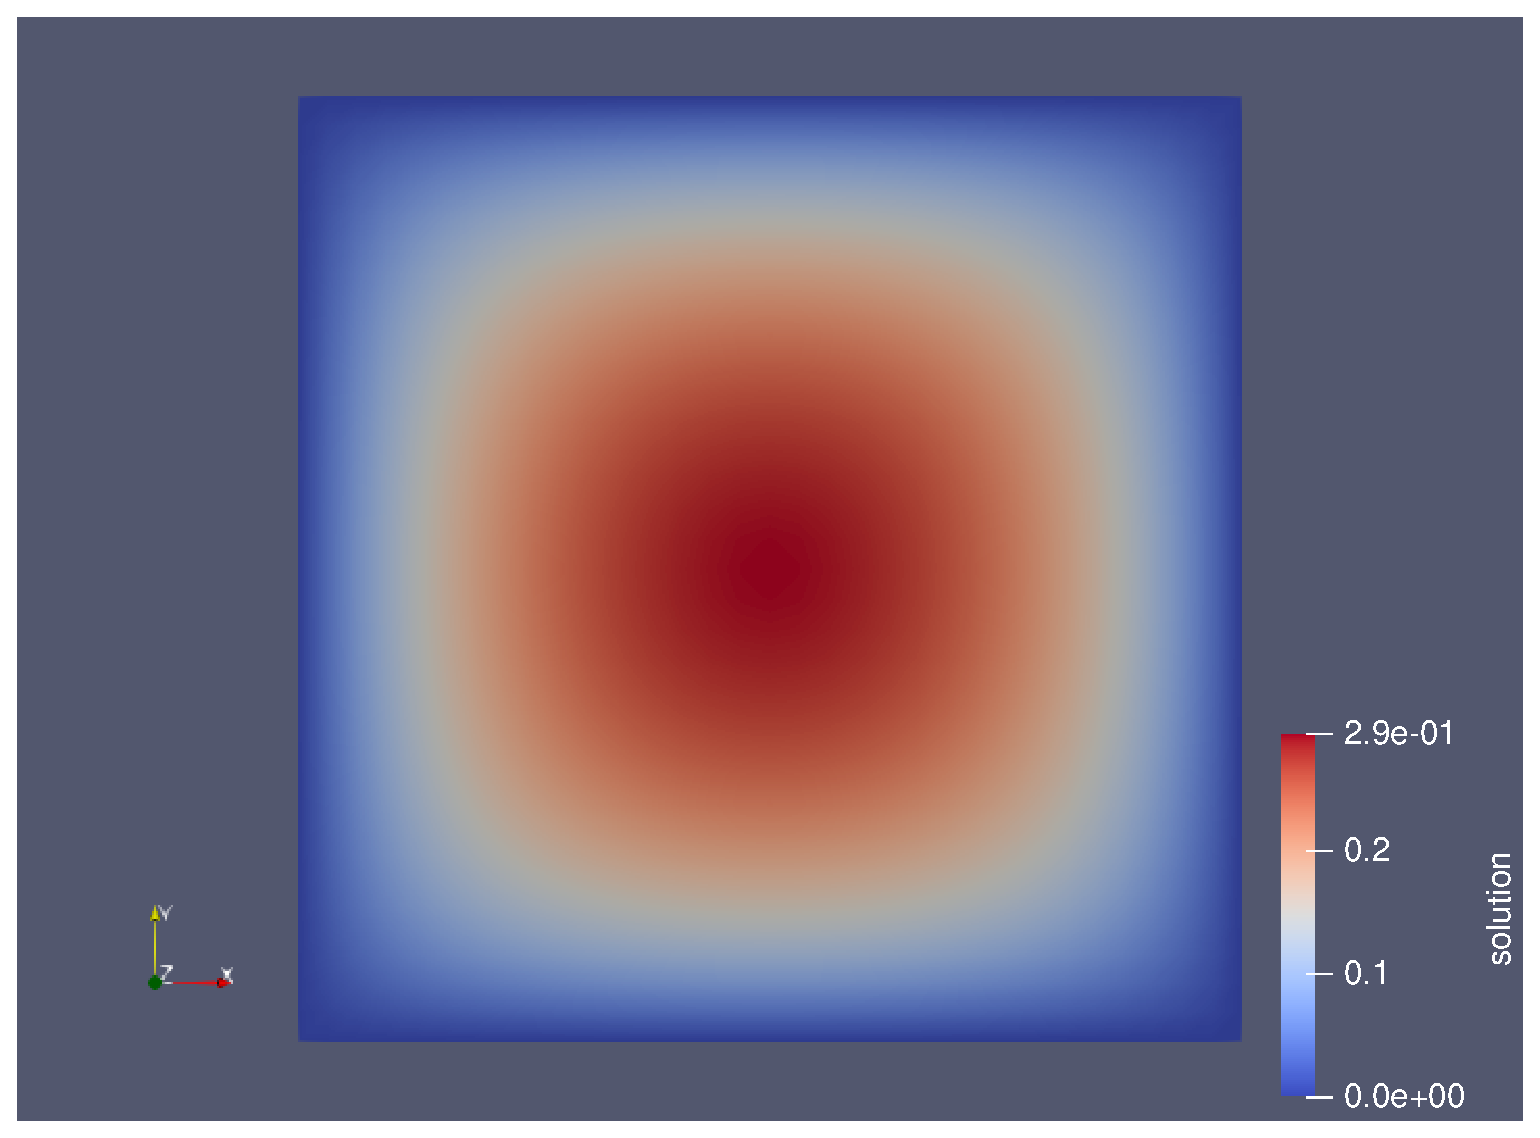
\includegraphics[scale=0.5]{./solution.eps}
      \caption{graph}
  \end{figure}
\end{document}


